% Options for packages loaded elsewhere
\PassOptionsToPackage{unicode}{hyperref}
\PassOptionsToPackage{hyphens}{url}
%
\documentclass[
  letterpaper,
]{scrbook}

\usepackage{amsmath,amssymb}
\usepackage{iftex}
\ifPDFTeX
  \usepackage[T1]{fontenc}
  \usepackage[utf8]{inputenc}
  \usepackage{textcomp} % provide euro and other symbols
\else % if luatex or xetex
  \usepackage{unicode-math}
  \defaultfontfeatures{Scale=MatchLowercase}
  \defaultfontfeatures[\rmfamily]{Ligatures=TeX,Scale=1}
\fi
\usepackage{lmodern}
\ifPDFTeX\else  
    % xetex/luatex font selection
  \setmainfont[]{Pretendard Regular}
\fi
% Use upquote if available, for straight quotes in verbatim environments
\IfFileExists{upquote.sty}{\usepackage{upquote}}{}
\IfFileExists{microtype.sty}{% use microtype if available
  \usepackage[]{microtype}
  \UseMicrotypeSet[protrusion]{basicmath} % disable protrusion for tt fonts
}{}
\makeatletter
\@ifundefined{KOMAClassName}{% if non-KOMA class
  \IfFileExists{parskip.sty}{%
    \usepackage{parskip}
  }{% else
    \setlength{\parindent}{0pt}
    \setlength{\parskip}{6pt plus 2pt minus 1pt}}
}{% if KOMA class
  \KOMAoptions{parskip=half}}
\makeatother
\usepackage{xcolor}
\setlength{\emergencystretch}{3em} % prevent overfull lines
\setcounter{secnumdepth}{5}
% Make \paragraph and \subparagraph free-standing
\ifx\paragraph\undefined\else
  \let\oldparagraph\paragraph
  \renewcommand{\paragraph}[1]{\oldparagraph{#1}\mbox{}}
\fi
\ifx\subparagraph\undefined\else
  \let\oldsubparagraph\subparagraph
  \renewcommand{\subparagraph}[1]{\oldsubparagraph{#1}\mbox{}}
\fi

\usepackage{color}
\usepackage{fancyvrb}
\newcommand{\VerbBar}{|}
\newcommand{\VERB}{\Verb[commandchars=\\\{\}]}
\DefineVerbatimEnvironment{Highlighting}{Verbatim}{commandchars=\\\{\}}
% Add ',fontsize=\small' for more characters per line
\usepackage{framed}
\definecolor{shadecolor}{RGB}{241,243,245}
\newenvironment{Shaded}{\begin{snugshade}}{\end{snugshade}}
\newcommand{\AlertTok}[1]{\textcolor[rgb]{0.68,0.00,0.00}{#1}}
\newcommand{\AnnotationTok}[1]{\textcolor[rgb]{0.37,0.37,0.37}{#1}}
\newcommand{\AttributeTok}[1]{\textcolor[rgb]{0.40,0.45,0.13}{#1}}
\newcommand{\BaseNTok}[1]{\textcolor[rgb]{0.68,0.00,0.00}{#1}}
\newcommand{\BuiltInTok}[1]{\textcolor[rgb]{0.00,0.23,0.31}{#1}}
\newcommand{\CharTok}[1]{\textcolor[rgb]{0.13,0.47,0.30}{#1}}
\newcommand{\CommentTok}[1]{\textcolor[rgb]{0.37,0.37,0.37}{#1}}
\newcommand{\CommentVarTok}[1]{\textcolor[rgb]{0.37,0.37,0.37}{\textit{#1}}}
\newcommand{\ConstantTok}[1]{\textcolor[rgb]{0.56,0.35,0.01}{#1}}
\newcommand{\ControlFlowTok}[1]{\textcolor[rgb]{0.00,0.23,0.31}{#1}}
\newcommand{\DataTypeTok}[1]{\textcolor[rgb]{0.68,0.00,0.00}{#1}}
\newcommand{\DecValTok}[1]{\textcolor[rgb]{0.68,0.00,0.00}{#1}}
\newcommand{\DocumentationTok}[1]{\textcolor[rgb]{0.37,0.37,0.37}{\textit{#1}}}
\newcommand{\ErrorTok}[1]{\textcolor[rgb]{0.68,0.00,0.00}{#1}}
\newcommand{\ExtensionTok}[1]{\textcolor[rgb]{0.00,0.23,0.31}{#1}}
\newcommand{\FloatTok}[1]{\textcolor[rgb]{0.68,0.00,0.00}{#1}}
\newcommand{\FunctionTok}[1]{\textcolor[rgb]{0.28,0.35,0.67}{#1}}
\newcommand{\ImportTok}[1]{\textcolor[rgb]{0.00,0.46,0.62}{#1}}
\newcommand{\InformationTok}[1]{\textcolor[rgb]{0.37,0.37,0.37}{#1}}
\newcommand{\KeywordTok}[1]{\textcolor[rgb]{0.00,0.23,0.31}{#1}}
\newcommand{\NormalTok}[1]{\textcolor[rgb]{0.00,0.23,0.31}{#1}}
\newcommand{\OperatorTok}[1]{\textcolor[rgb]{0.37,0.37,0.37}{#1}}
\newcommand{\OtherTok}[1]{\textcolor[rgb]{0.00,0.23,0.31}{#1}}
\newcommand{\PreprocessorTok}[1]{\textcolor[rgb]{0.68,0.00,0.00}{#1}}
\newcommand{\RegionMarkerTok}[1]{\textcolor[rgb]{0.00,0.23,0.31}{#1}}
\newcommand{\SpecialCharTok}[1]{\textcolor[rgb]{0.37,0.37,0.37}{#1}}
\newcommand{\SpecialStringTok}[1]{\textcolor[rgb]{0.13,0.47,0.30}{#1}}
\newcommand{\StringTok}[1]{\textcolor[rgb]{0.13,0.47,0.30}{#1}}
\newcommand{\VariableTok}[1]{\textcolor[rgb]{0.07,0.07,0.07}{#1}}
\newcommand{\VerbatimStringTok}[1]{\textcolor[rgb]{0.13,0.47,0.30}{#1}}
\newcommand{\WarningTok}[1]{\textcolor[rgb]{0.37,0.37,0.37}{\textit{#1}}}

\providecommand{\tightlist}{%
  \setlength{\itemsep}{0pt}\setlength{\parskip}{0pt}}\usepackage{longtable,booktabs,array}
\usepackage{calc} % for calculating minipage widths
% Correct order of tables after \paragraph or \subparagraph
\usepackage{etoolbox}
\makeatletter
\patchcmd\longtable{\par}{\if@noskipsec\mbox{}\fi\par}{}{}
\makeatother
% Allow footnotes in longtable head/foot
\IfFileExists{footnotehyper.sty}{\usepackage{footnotehyper}}{\usepackage{footnote}}
\makesavenoteenv{longtable}
\usepackage{graphicx}
\makeatletter
\def\maxwidth{\ifdim\Gin@nat@width>\linewidth\linewidth\else\Gin@nat@width\fi}
\def\maxheight{\ifdim\Gin@nat@height>\textheight\textheight\else\Gin@nat@height\fi}
\makeatother
% Scale images if necessary, so that they will not overflow the page
% margins by default, and it is still possible to overwrite the defaults
% using explicit options in \includegraphics[width, height, ...]{}
\setkeys{Gin}{width=\maxwidth,height=\maxheight,keepaspectratio}
% Set default figure placement to htbp
\makeatletter
\def\fps@figure{htbp}
\makeatother
% definitions for citeproc citations
\NewDocumentCommand\citeproctext{}{}
\NewDocumentCommand\citeproc{mm}{%
  \begingroup\def\citeproctext{#2}\cite{#1}\endgroup}
\makeatletter
 % allow citations to break across lines
 \let\@cite@ofmt\@firstofone
 % avoid brackets around text for \cite:
 \def\@biblabel#1{}
 \def\@cite#1#2{{#1\if@tempswa , #2\fi}}
\makeatother
\newlength{\cslhangindent}
\setlength{\cslhangindent}{1.5em}
\newlength{\csllabelwidth}
\setlength{\csllabelwidth}{3em}
\newenvironment{CSLReferences}[2] % #1 hanging-indent, #2 entry-spacing
 {\begin{list}{}{%
  \setlength{\itemindent}{0pt}
  \setlength{\leftmargin}{0pt}
  \setlength{\parsep}{0pt}
  % turn on hanging indent if param 1 is 1
  \ifodd #1
   \setlength{\leftmargin}{\cslhangindent}
   \setlength{\itemindent}{-1\cslhangindent}
  \fi
  % set entry spacing
  \setlength{\itemsep}{#2\baselineskip}}}
 {\end{list}}
\usepackage{calc}
\newcommand{\CSLBlock}[1]{\hfill\break\parbox[t]{\linewidth}{\strut\ignorespaces#1\strut}}
\newcommand{\CSLLeftMargin}[1]{\parbox[t]{\csllabelwidth}{\strut#1\strut}}
\newcommand{\CSLRightInline}[1]{\parbox[t]{\linewidth - \csllabelwidth}{\strut#1\strut}}
\newcommand{\CSLIndent}[1]{\hspace{\cslhangindent}#1}

% load packages
\usepackage{fontspec}
\makeatletter
\@ifpackageloaded{tcolorbox}{}{\usepackage[skins,breakable]{tcolorbox}}
\@ifpackageloaded{fontawesome5}{}{\usepackage{fontawesome5}}
\definecolor{quarto-callout-color}{HTML}{909090}
\definecolor{quarto-callout-note-color}{HTML}{0758E5}
\definecolor{quarto-callout-important-color}{HTML}{CC1914}
\definecolor{quarto-callout-warning-color}{HTML}{EB9113}
\definecolor{quarto-callout-tip-color}{HTML}{00A047}
\definecolor{quarto-callout-caution-color}{HTML}{FC5300}
\definecolor{quarto-callout-color-frame}{HTML}{acacac}
\definecolor{quarto-callout-note-color-frame}{HTML}{4582ec}
\definecolor{quarto-callout-important-color-frame}{HTML}{d9534f}
\definecolor{quarto-callout-warning-color-frame}{HTML}{f0ad4e}
\definecolor{quarto-callout-tip-color-frame}{HTML}{02b875}
\definecolor{quarto-callout-caution-color-frame}{HTML}{fd7e14}
\makeatother
\makeatletter
\@ifpackageloaded{bookmark}{}{\usepackage{bookmark}}
\makeatother
\makeatletter
\@ifpackageloaded{caption}{}{\usepackage{caption}}
\AtBeginDocument{%
\ifdefined\contentsname
  \renewcommand*\contentsname{Table of contents}
\else
  \newcommand\contentsname{Table of contents}
\fi
\ifdefined\listfigurename
  \renewcommand*\listfigurename{List of Figures}
\else
  \newcommand\listfigurename{List of Figures}
\fi
\ifdefined\listtablename
  \renewcommand*\listtablename{List of Tables}
\else
  \newcommand\listtablename{List of Tables}
\fi
\ifdefined\figurename
  \renewcommand*\figurename{Figure}
\else
  \newcommand\figurename{Figure}
\fi
\ifdefined\tablename
  \renewcommand*\tablename{Table}
\else
  \newcommand\tablename{Table}
\fi
}
\@ifpackageloaded{float}{}{\usepackage{float}}
\floatstyle{ruled}
\@ifundefined{c@chapter}{\newfloat{codelisting}{h}{lop}}{\newfloat{codelisting}{h}{lop}[chapter]}
\floatname{codelisting}{Listing}
\newcommand*\listoflistings{\listof{codelisting}{List of Listings}}
\makeatother
\makeatletter
\makeatother
\makeatletter
\@ifpackageloaded{caption}{}{\usepackage{caption}}
\@ifpackageloaded{subcaption}{}{\usepackage{subcaption}}
\makeatother
\ifLuaTeX
  \usepackage{selnolig}  % disable illegal ligatures
\fi
\usepackage{bookmark}

\IfFileExists{xurl.sty}{\usepackage{xurl}}{} % add URL line breaks if available
\urlstyle{same} % disable monospaced font for URLs
\hypersetup{
  pdftitle={Where Learnings Come Together},
  pdfauthor={Jonghwan Yoon},
  hidelinks,
  pdfcreator={LaTeX via pandoc}}

\title{Where Learnings Come Together}
\author{Jonghwan Yoon}
\date{2024-09-17}

\begin{document}
\frontmatter
\maketitle

\renewcommand*\contentsname{Table of contents}
{
\setcounter{tocdepth}{2}
\tableofcontents
}
\mainmatter
\bookmarksetup{startatroot}

\chapter*{Preface}\label{preface}
\addcontentsline{toc}{chapter}{Preface}

\markboth{Preface}{Preface}

여러가지 내용을 정리하는 곳.

\part{Computer Science}

\chapter{성능평가에 사용할 수 있는
도구들}\label{uxc131uxb2a5uxd3c9uxac00uxc5d0-uxc0acuxc6a9uxd560-uxc218-uxc788uxb294-uxb3c4uxad6cuxb4e4}

정리 중.

\section*{time}\label{time}
\addcontentsline{toc}{section}{time}

\markright{time}

(MacKenzie 1996)

\texttt{time}은 shell keyword이다. 여기서 소개하는 것은
\texttt{/usr/bin/time}에 해당하는 것으로 \textbf{shell에 내장된
keyword가 아닌 GNU의 \texttt{time}}이다.

\begin{Shaded}
\begin{Highlighting}[]
\ExtensionTok{/usr/bin/time} \AttributeTok{{-}v}\NormalTok{ sleep 1s}
\end{Highlighting}
\end{Shaded}

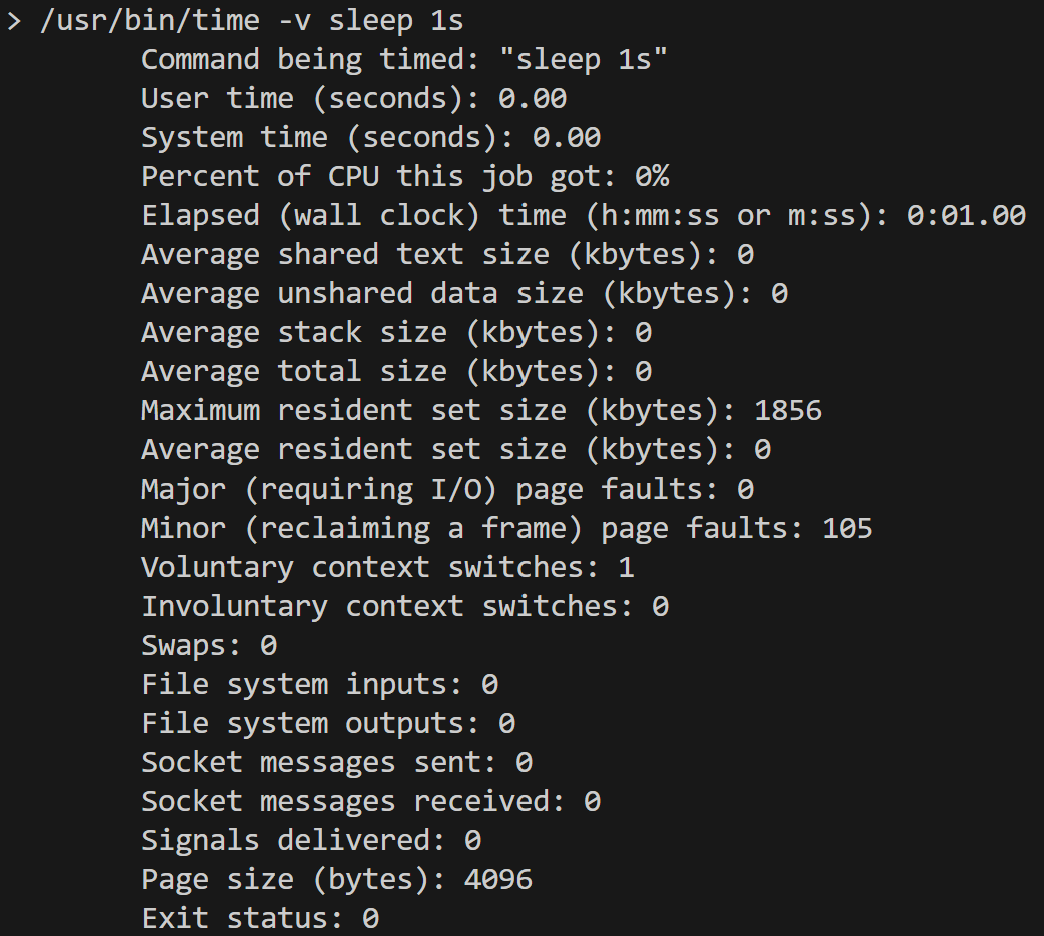
\includegraphics[width=0.7\textwidth,height=\textheight]{chapters/ComputerScience/benchmarking/time_v.png}

\begin{itemize}
\tightlist
\item
  장점: 상세하다. computing resource도 계산해준다.
\item
  단점: unix 계열 아니면 사용할 수 없음.
\end{itemize}

\begin{tcolorbox}[enhanced jigsaw, opacityback=0, bottomrule=.15mm, toptitle=1mm, colback=white, colframe=quarto-callout-tip-color-frame, breakable, colbacktitle=quarto-callout-tip-color!10!white, opacitybacktitle=0.6, bottomtitle=1mm, left=2mm, coltitle=black, titlerule=0mm, rightrule=.15mm, title=\textcolor{quarto-callout-tip-color}{\faLightbulb}\hspace{0.5em}{TMI}, arc=.35mm, toprule=.15mm, leftrule=.75mm]

\begin{itemize}
\tightlist
\item
  GNU time은 2017년부터 \texttt{Assaf\ Gordon} 라는 분이 관리했는데
  Bioinformatics를 하시는 분이다.👀
\item
  \texttt{which\ time}도 \texttt{/usr/bin/time}을 출력하는데, 그냥
  path에 같이 있어서 그렇다. shell keyword로 대상으로 which를 하면 fail
  code를 반환한다.
\end{itemize}

\end{tcolorbox}

\section*{hyperfine}\label{hyperfine}
\addcontentsline{toc}{section}{hyperfine}

\markright{hyperfine}

(Peter 2023)

\href{https://github.com/sharkdp/hyperfine}{github}

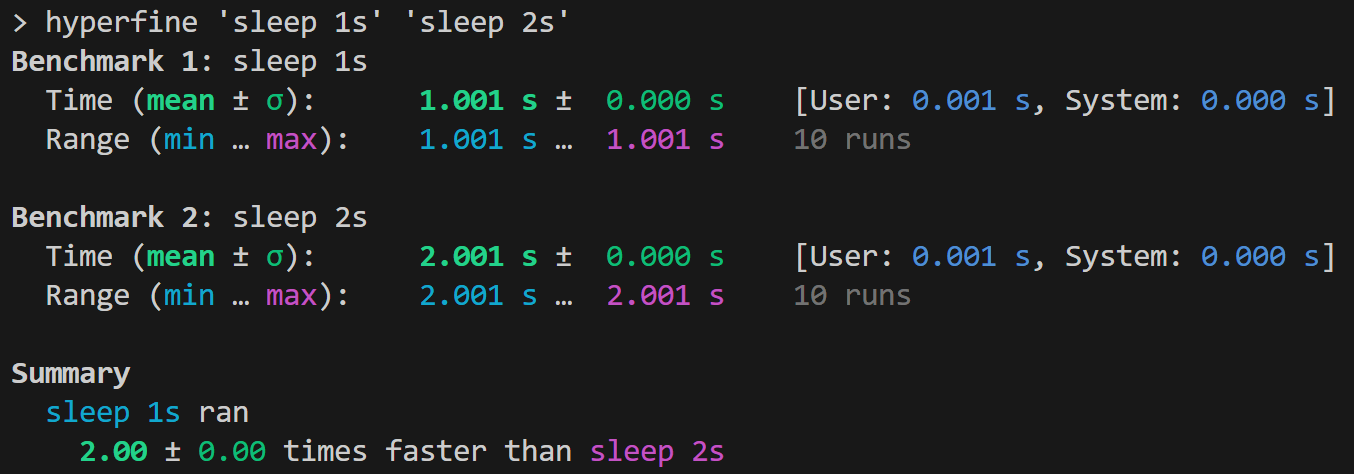
\includegraphics{chapters/ComputerScience/benchmarking/hyperfine_example.png}

\begin{itemize}
\tightlist
\item
  장점: 간단하다. 이쁘고 보기좋게 측정해준다.
\item
  단점: CPU, Memory usage는 계산하지 못하는듯.
\end{itemize}

이쁜 timeit 느낌.

\part{Bioinformatics}

test

\part{Programming}

\part{Rust}

\chapter{noodles::bam}\label{noodlesbam}

noodles (zaeleus 2018) 는 생물정보학 관련 데이터를 다루기 위해 만들어진
순수 rust로 작성된 Crate이다.
(\href{https://github.com/zaeleus/noodles}{github})

그 중, BAM 파일을 다루는 noodles::bam에 대해서 bam파일을 읽고 쓰는
방법에 대해 정리한다. pysam과 비교하며 진행한다.

\part{Godot}

\part{Godot-Rust}

\part{기타}

\chapter{Quarto의 Citation Style}\label{quartouxc758-citation-style}

문헌을 작성할 때, 참고자료를 citation을 한다.

LaTex 문서에서 \texttt{.bib} 파일은 참고문헌을 정리하기 위한
\textbf{BibLaTeX} 파일이다. 여기에 참고문헌 정보가 정리되고 LaTex에서
참고문헌 목록을 자동으로 생성하는데 사용된다.

Quarto 에서도 참고문헌 문서화에 \texttt{.bib} 파일을 사용한다.

대략적인 정보는 다음
\href{https://quarto.org/docs/authoring/citations.html\#sec-citations-style}{링크}에
있다.

여기서는 링크에서 다루지 않는 \texttt{.bib} 파일에 사용되는 문헌 포맷과
CSL 스타일을 정리한다. 기본 세팅은 다루지 않는다.

\section{\texorpdfstring{\texttt{.bib} 파일
구조}{.bib 파일 구조}}\label{bib-uxd30cuxc77c-uxad6cuxc870}

해당 파일에는 문헌 별 자료가 존재하는데 이를 entry라고 한다.

각 엔트리는 \texttt{@type\{uniqueID\}} 형식으로 표현된다. 문헌의 고유한
이름은 \texttt{uniqueID} 로 표시되고, 문헌 정보는 key=\{value\} 형식으로
입력된다.

주요 타입은 다음과 같다.

\begin{itemize}
\tightlist
\item
  \texttt{@article}: 논문을 인용할 때 사용
\item
  \texttt{@book}: 책을 인용할 때 사용
\item
  \texttt{@inproceedings}: 학회 발표 논문
\item
  \texttt{@software}: 소프트웨어 인용시 사용.
\item
  \texttt{@manual}: 사용자 가이드 같은 매뉴얼에 사용.
\item
  \texttt{@misc}: 다양한 출처 (예: 웹사이트) 인용 시 사용
\end{itemize}

기타 타입은 다음과 같다.

\begin{itemize}
\tightlist
\item
  \texttt{@inbook}
\item
  \texttt{@incollection}
\item
  \texttt{@phdthesis}, \texttt{@masterthesis}
\end{itemize}

예를 들면 아래와 같다.

\begin{Shaded}
\begin{Highlighting}[]
\VariableTok{@article}\NormalTok{\{}\OtherTok{knuth:1984}\NormalTok{,}
  \DataTypeTok{title}\NormalTok{=\{Literate Programming\},}
  \DataTypeTok{author}\NormalTok{=\{Donald E. Knuth\},}
  \DataTypeTok{journal}\NormalTok{=\{The Computer Journal\},}
  \DataTypeTok{volume}\NormalTok{=\{27\},}
  \DataTypeTok{number}\NormalTok{=\{2\},}
  \DataTypeTok{pages}\NormalTok{=\{97{-}{-}111\},}
  \DataTypeTok{year}\NormalTok{=\{1984\},}
  \DataTypeTok{publisher}\NormalTok{=\{Oxford University Press\}}
\NormalTok{\}}
\end{Highlighting}
\end{Shaded}

위 고유 ID는 \texttt{knuth:1984}이다. qmd 파일에 \texttt{@knuth:1984}를
입력하면 다음처럼 나타난다.

➡️ Knuth (1984)

괄호에 따라 몇가지 변형이 있다.

\begin{itemize}
\tightlist
\item
  \texttt{{[}@knuth:1984{]}}: (Knuth 1984)
\end{itemize}

기본 세팅은
\href{https://www.chicagomanualofstyle.org/home.html}{Chicago Manual fo
Style}을 따른다. quarto에서 포맷을 바꾸고 싶다면 CSL 파일을
제공해야한다.

\section{Citation Style Language (CSL)
파일}\label{citation-style-language-csl-uxd30cuxc77c}

csl 파일은 citation을 어떻게 표현할지에 대한 포맷이 작성된 XML 파일이다.

직접수정하기는 어려울 수 있다.

하지만 만들어진 csl 파일이 정말많으므로 원하는 포맷을 검색하는게 더
낫다.

\href{https://editor.citationstyles.org/searchByExample/}{CSL에서
제공하는 style seacrh engine}

citation 구조를 바꾸기 위해서는 \textbf{Citation Style Language}를
주어야 한다. \texttt{.csl} 파일을 제공해야 하며 파일이 있을 때 적용하는
방법은
\href{https://quarto.org/docs/authoring/citations.html\#sec-citations-style}{링크}
에 있다.

\bookmarksetup{startatroot}

\chapter*{References}\label{references}
\addcontentsline{toc}{chapter}{References}

\markboth{References}{References}

\phantomsection\label{refs}
\begin{CSLReferences}{1}{0}
\bibitem[\citeproctext]{ref-knuth:1984}
Knuth, Donald E. 1984. {``Literate Programming.''} \emph{The Computer
Journal} 27 (2): 97--111.

\bibitem[\citeproctext]{ref-gnu_bash_time}
MacKenzie, David. 1996. \emph{Time}. GNU Project; Online.
\url{https://man7.org/linux/man-pages/man1/time.1.html}.

\bibitem[\citeproctext]{ref-Peter_hyperfine_2023}
Peter, David. 2023. {``{hyperfine}.''}
\url{https://github.com/sharkdp/hyperfine}.

\bibitem[\citeproctext]{ref-github:noodles}
zaeleus. 2018. {``Noodles.''} \url{https://github.com/zaeleus/noodles}.

\end{CSLReferences}


\backmatter

\end{document}
